\documentclass{report}

\usepackage{amsmath}
\usepackage{amssymb}
\usepackage[pdftex]{graphicx}
\usepackage{epstopdf}
\usepackage{enumerate}  % for enumerating with a), b) etc...
\usepackage{caption}    % for having enumertion in a caption 
\usepackage[]{algorithm2e}
\usepackage[margin=1in]{geometry}

\graphicspath{ {./} {Figures/}}

\begin{document}

The system
\begin{align}
    M_t &= \nabla_x \left( D(M) \nabla_x M \right) + f(C,M) M \\
    C_t &= - y g(C) M 
\end{align}
where
\begin{align}
    D(M) &= \delta \frac{M^\alpha}{(1 - M)^\beta} \\
    f(C,M) &= g(C) - \frac{y}{10} \\
    g(C,M) &= \frac{C}{k +C}
\end{align}
is solved on a rectangular region with length $L$ and width $\lambda L$ with the following parameter values,
\begin{equation}
\begin{aligned}
    L &= 0.01 \\
    \lambda &= \frac{1}{128}\\
    \alpha &= 4 \\
    \beta &= 4 \\
    \mu &= 6 \\      
\end{aligned}
\qquad
\begin{aligned}
    C_0 &= 30 \\
    M_0 &= 30 \\
    \delta &= \frac{10^{-7}}{\mu L^2} \approx 10^-4\\
    k &= \frac{4}{C_0} \approx 0.1333\\
    \nu &= \frac{M_0}{0.63 \cdot C_0} \approx 1.59,\\
\end{aligned}
\end{equation}
and with initial conditions 
\begin{equation}
\begin{aligned}
    C &= 1 \\
    M &= \begin{cases} -(\frac{h}{d^4})x^4 + h & \text{if } x < 0.04 \\ 0 & \text{otherwise }\end{cases} \\
\end{aligned}
\end{equation}  
where $h = 0.1, d=\frac{5}{128}$ , representing the height and depth of the inoculation site.

Using simulation code version $0.6$ the possibilty of a travelling wave solution existing was examined. The following results were found using a finite difference method to solve $M$ and trapizedral rule to solve $C$ with $\Delta x = \frac{1}{8192}$ and $\Delta t = 10^-2$.

The solution to the above system can be seen in Figure \ref{fig:solution}. This solution seems to have characteristics of a travelling wave solution. This is because after $t=70$, we can write the solution $M(x,t)$ as $M(x-ct)$, where $c$ is the wavespeed of the solution. We can numerically approximate the value for $c$ by looking at how fast the peak of the wave travels, Figure \ref{fig:waveSpeed} shows that this value is $c \approx c^n = 1/440$. Now we can show that the solutions can be written as $M(x-ct)$ by shifting solutions of $M(x,t)$ by $\pm n_i c$, with $n_i \in \mathbb{Z}$, as seen in Figure \ref{fig:travShape}.


\begin{figure}[h!tb]
\begin{center}
  \begin{tabular}{c c}
      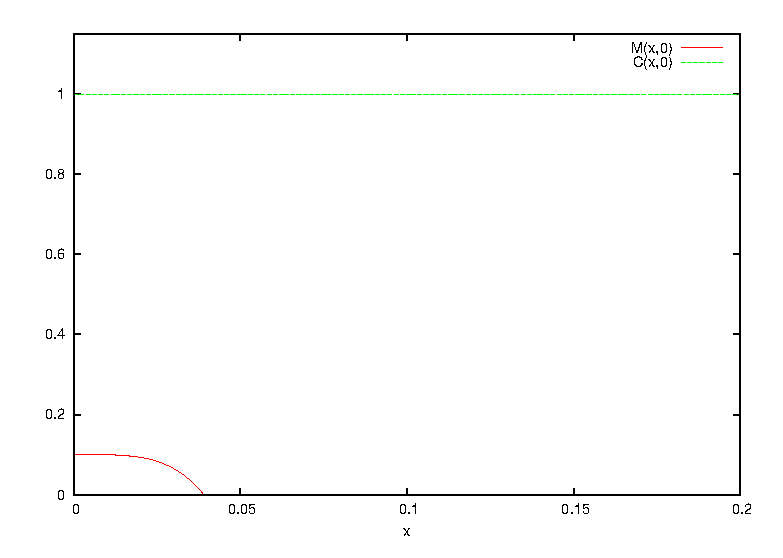
\includegraphics[scale=0.55]{solution_t0.eps} &
      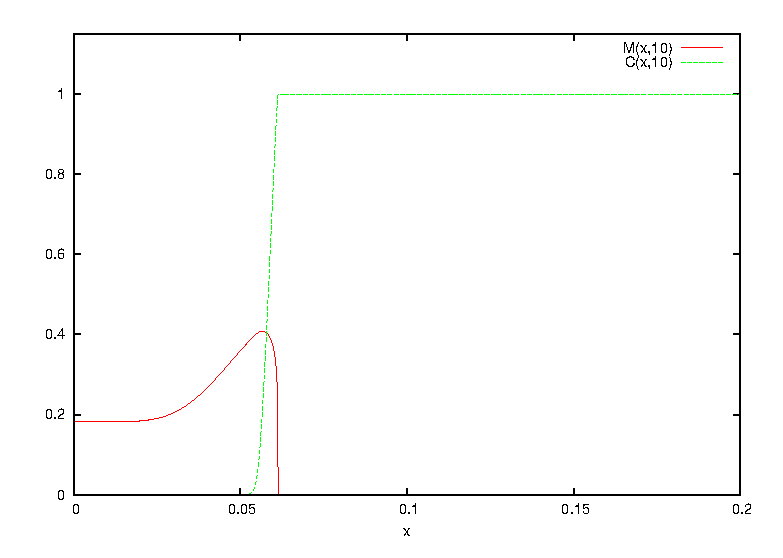
\includegraphics[scale=0.55]{solution_t10.eps} \\
      (a) & (b) \\
      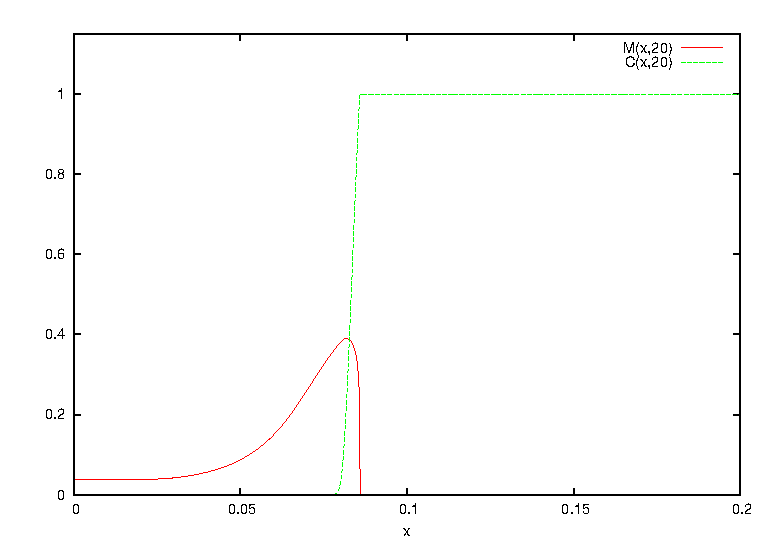
\includegraphics[scale=0.55]{solution_t20.eps} &
      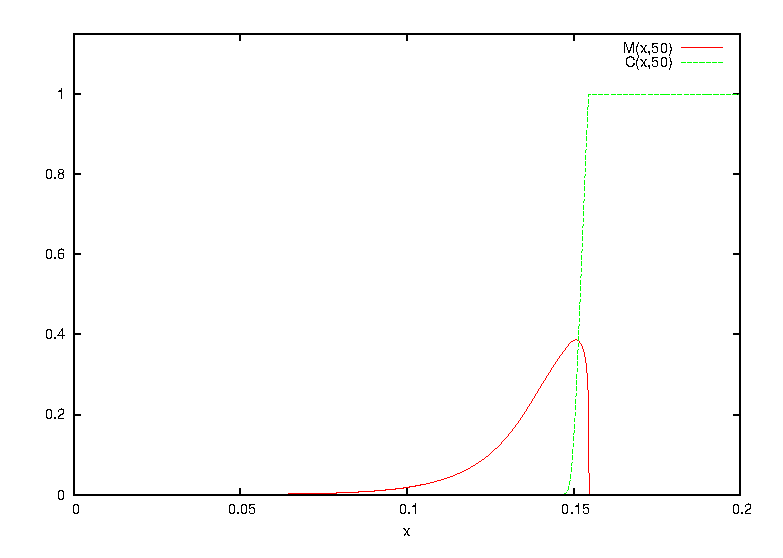
\includegraphics[scale=0.55]{solution_t50.eps} \\
      (c) & (d) 
  \end{tabular}
  \caption{Solutions of $M(x,t)$ and $C(x,t)$ at (a) t = 0, (b) t = 10, (c) = 20, (d) = 50. }
  \label{fig:solution}
\end{center}
\end{figure}

\begin{figure}[h!tb]
\begin{center}
    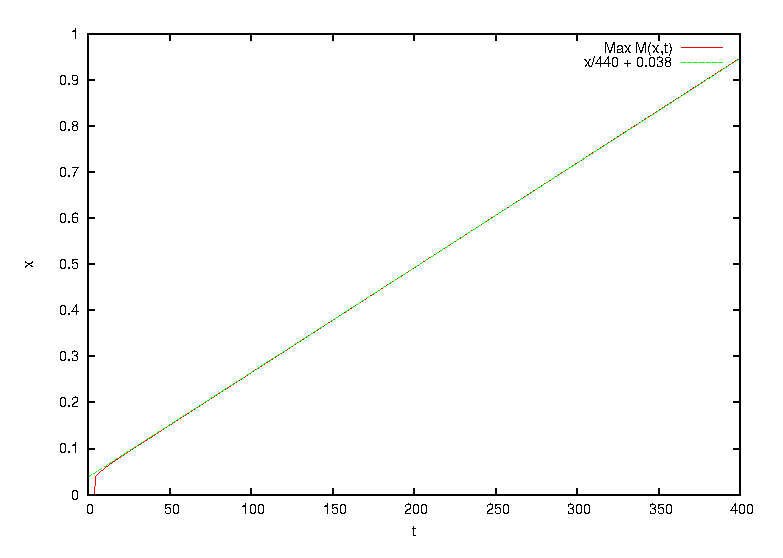
\includegraphics[scale=0.85]{wavespeed.eps}
    \caption{Max $M$ value as a function of $t$. The green line is an approximation for the wavespeed, $c$.}
    \label{fig:waveSpeed} 
\end{center}
\end{figure}

\begin{figure}[h!tb]
\begin{center}
    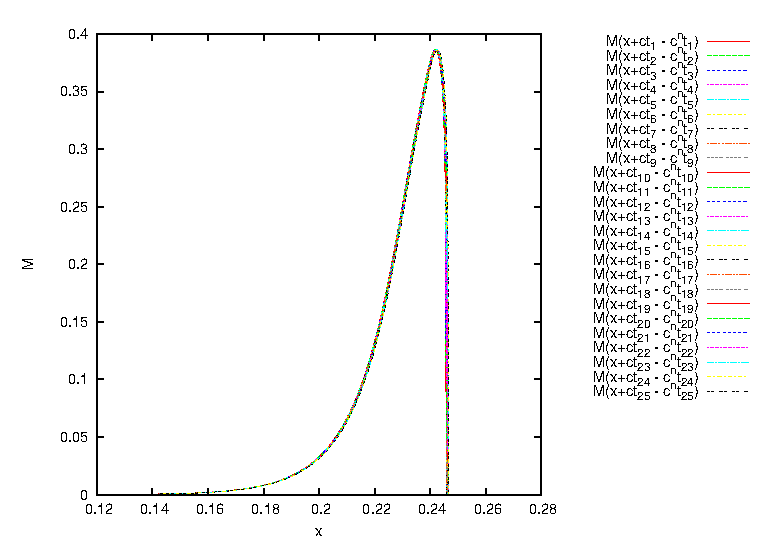
\includegraphics[scale=0.85]{travShape.eps}
    \caption{Solutions of $M(x+ct)$ at time $t_i = 1 \ldots 25$ each horizontally translated by $-n_i c^n$, where $n_i = 1 \ldots 25$ and $c^n = 1/440$}
    \label{fig:travShape}
\end{center}
\end{figure}

\end{document}



